\documentclass[a4paper,11pt]{article}
\usepackage[utf8]{inputenc}
\usepackage[english]{babel}
\usepackage[vmargin=4.0cm]{geometry}
\usepackage[linktocpage=true]{hyperref}
\usepackage[ddmmyyyy]{datetime}
\usepackage{pdfpages}
\usepackage{framed}
\renewcommand{\dateseparator}{.}
\usepackage{watermark}

\hypersetup{
    colorlinks,
    citecolor=black,
    filecolor=black,
    linkcolor=black,
    urlcolor=black
}

\usepackage{listings}% http://ctan.org/pkg/listings
\usepackage{xcolor}% http://ctan.org/pkg/xcolor
\definecolor{bluekeywords}{rgb}{0.13,0.13,1}
\definecolor{greencomments}{rgb}{0,0.5,0}
\definecolor{turqusnumbers}{rgb}{0.17,0.57,0.69}
\definecolor{redstrings}{rgb}{0.5,0,0}
\definecolor{graybg}{rgb}{0.92,0.92,0.92}

\lstdefinelanguage{FSharp}
    {morekeywords={let, new, match, with, rec, open, module, namespace, type, of, member, and, for, in, do, begin, end, fun, function, try, mutable, if, then, else},
    keywordstyle=\color{bluekeywords},
    sensitive=false,
    morecomment=[l][\color{greencomments}]{///},
    morecomment=[l][\color{greencomments}]{//},
    morecomment=[s][\color{greencomments}]{{(*}{*)}},
    morestring=[b]",
    stringstyle=\color{redstrings}
    }

\lstnewenvironment{fs}
  {
    \lstset{
        language=FSharp,
        basicstyle=\ttfamily,
        breaklines=true,
        numbers=left,
        columns=fullflexible,
        frame=single}
  }
  {
  }
\lstdefinestyle{customc}{
  belowcaptionskip=1\baselineskip,
  breaklines=true,
  frame=L,
  language=C,
  showstringspaces=false,
  basicstyle=\footnotesize\ttfamily,
  keywordstyle=\bfseries\color{green!40!black},
  commentstyle=\itshape\color{purple!40!black},
  identifierstyle=\color{blue},
  stringstyle=\color{orange},
}
\lstnewenvironment{ccode}
  {
    \lstset{
        language=C,
        basicstyle=\ttfamily,
        breaklines=true,
        numbers=left,
        frame=single,
        columns=fullflexible}
  }
  {
  }
\lstnewenvironment{bashcode}
  {
    \lstset{
        language=make,
        basicstyle=\ttfamily,
        breaklines=true,
        numbers=left,
        frame=single,
        columns=fullflexible}
  }
  {
  }

\begin{document}
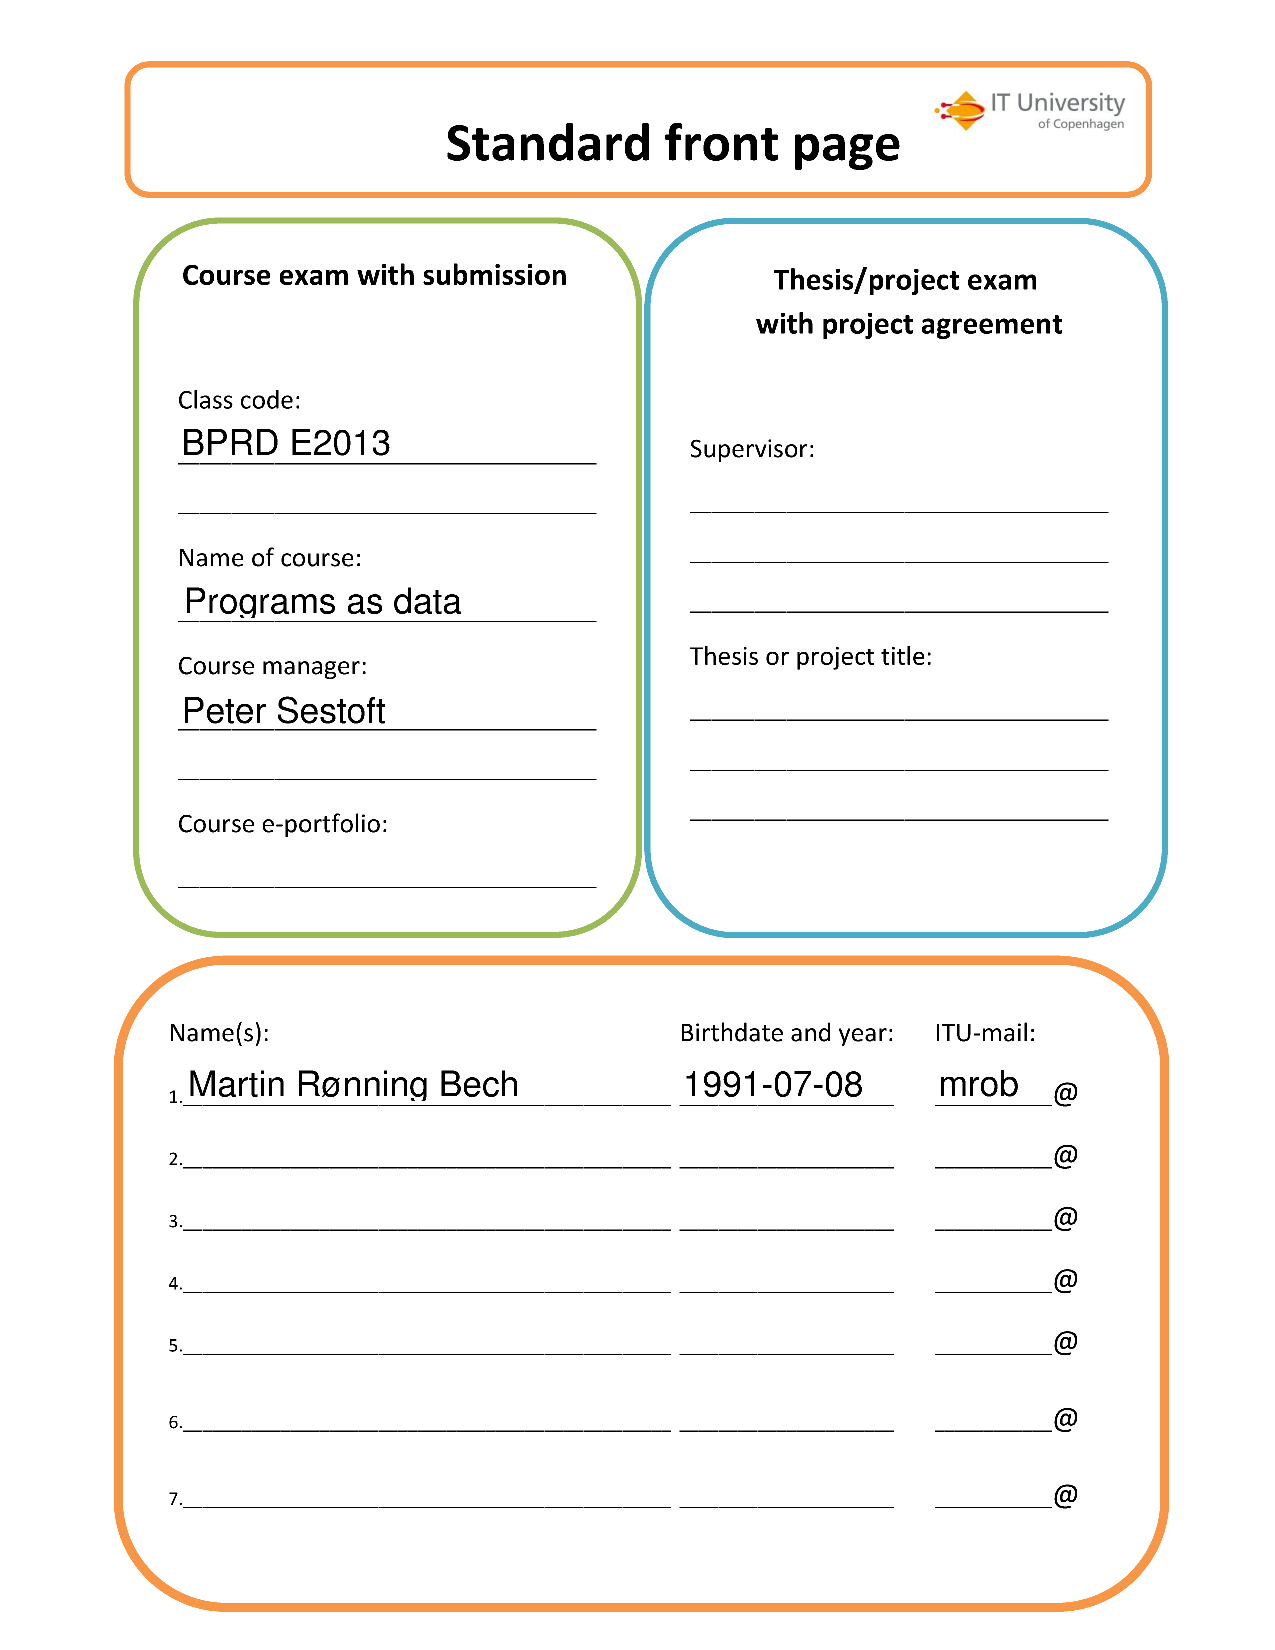
\includepdf{formal/forside.pdf}
\begin{titlepage}
\begin{flushleft}
\textbf{Course:} Programs as data - E2013
\end{flushleft}
\vspace{30mm}
\centering \parindent=0pt
\Huge\bfseries
Programs as data\\[0.7cm]
\large Eksamens aflevering\\
\vspace{20mm}
    Martin Rønning Bech 
\\  mrob@itu.dk\\
\vspace{50mm}
Date: \today

\vspace{25mm}
%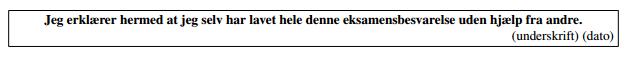
\includegraphics[width=1.1\textwidth]{formal/sign.png}
\begin{framed}
    \begin{minipage}{1\textwidth}
        \textbf{Jeg erklærer hermed at jeg selv har lavet hele denne
        eksamensbesvarelse uden hjælp fra andre.}
        \begin{flushright}
            (underskrift) (dato)
        \end{flushright}
    \end{minipage}
\end{framed}


\end{titlepage}

\section{Opgave 1}
\subsection{Implementation}
CLex.fsl
\begin{fs}
let keyword s =
    match s with
    ...
    | "for"     -> FOR
    | "to"      -> TO
    | "do"      -> DO
    ...
\end{fs}
CPar.fsy
In the CPar.fsy file I have added the tokens FOR TO DO and in StmtU and StmtM I
have added the following code:
\begin{fs}
StmtM:
...
  | FOR NAME ASSIGN Expr TO Expr DO StmtM { Block[Dec(TypI, $2); Stmt(Expr(Assign(AccVar($2), $4))); Stmt(While(Prim2("<=", Access(AccVar($2)), $6), Block[Stmt($8);Stmt(Expr(Assign(AccVar($2), Prim2("+", Access(AccVar($2)), CstI(1)))))]))] }
...
StmtU:
  | FOR NAME ASSIGN Expr TO Expr DO StmtU { Block[Dec(TypI, $2); Stmt(Expr(Assign(AccVar($2), $4))); Stmt(While(Prim2("<=", Access(AccVar($2)), $6), Block[Stmt($8);Stmt(Expr(Assign(AccVar($2), Prim2("+", Access(AccVar($2)), CstI(1)))))]))] }
\end{fs}
\subsection{Test}
Below is my test example code. It uses the for-loop to print the numbers 0 - 10
and ends by printing a newline. Resulting in an output like the following:
\texttt{0 1 2 3 4 5 6 7 8 9 10}
\begin{ccode}
void main() {
  for i=0 to 10 do 
    print i;

  println;
}
\end{ccode}
\subsection{Result}
To run the example I use two extra file, one called mcc.fs and Makefile both can
be found in the appendix with a short description of what they do. With the two
files in the same directory as the MicroC code and the example code stored in
\texttt{examples} directory I can do the following to test my example:
\begin{bashcode}
make
./mcc.exe examples/ex1.c examples/ex1.out
javac Machine.java
java Machine examples/ex1.out
\end{bashcode}
This gives me the expect output of:
\begin{bashcode}
% java Machine examples/ex2.out
0 1 2 3 4 5 6 7 8 9 10

\end{bashcode}

\section{Opgave 2}
\subsection{Implementation}
CLex.fsl:
\begin{fs}
rule Token = parse
...
  | "+="            { PEQ }
  | "-="            { MEQ }
...
\end{fs}
CPar.fsy:
\begin{fs}
%token PEQ MEQ
...
%nonassoc GT LT GE LE
%nonassoc PEQ MEQ 
%left PLUS MINUS
...
ExprNotAccess:
...
  | Access PEQ Expr                     { PlusEq($1, $3)      } 
  | Access MEQ Expr                     { MinusEq($1, $3)     } 

\end{fs}
Absyn.fs:
\begin{fs}
and expr =                                                         
  | PlusEq of access * expr          (* x+=e or *p+=e or a[e]+=e    *)
  | MinusEq of access * expr         (* x-=e or *p-=e or a[e]-=e    *)
\end{fs}
Comp.fs:
\begin{fs}
and cExpr (e : expr) (varEnv : varEnv) (funEnv : funEnv) : instr list = 
...
    | PlusEq(acc, e)  -> cAccess acc varEnv funEnv @ [DUP] @ [LDI] @ cExpr e varEnv funEnv @ [ADD] @ [STI]
    | MinusEq(acc, e)  -> cAccess acc varEnv funEnv @ [DUP] @ [LDI] @ cExpr e varEnv funEnv @ [SUB] @ [STI]
\end{fs}

\subsection{Test}
\begin{ccode}
void main() {
    int arr[2];
    int i;
    i = 0;
    arr[0] = 10;
    arr[1] = 100;
    
    arr[i=i+1] += 100;
    print arr[0];
    print arr[1];
    print i;
    println;

    int j;
    j = 2;
    arr[j=j-1] -= 100;
    print arr[0];
    print arr[1];
    print j;
    println;
}
\end{ccode}
\subsection{Result}
The output is as expected:
\begin{bashcode}
% java Machine examples/ex2.out
10 200 1 
10 100 1
\end{bashcode}

\section{Opgave 3}
\subsection{Implemetation}
Machine.fs:
\begin{fs}
type instr =
    | INDEX 
...
let CODEINDEX  = 26
let makelabenv (addr, labenv) instr = 
    match instr with
    | INDEX          -> (addr+1, labenv)
...
let rec emitints getlab instr ints = 
    match instr with
    | INDEX          -> CODEINDEX  :: ints
...
\end{fs}
Machine.java:
\begin{ccode}
final static int INDEX = 26;
static int execcode(int[] p, int[] s, int[] iargs, boolean trace) {
...
    switch (p[pc++]) {
        case INDEX:
        int a = sp-2;
        int q = s[a];
        int n = a - q;
        int i = s[sp];
        if(0 <= i && i < n){
            s[sp-1] = s[s[sp-1]]+s[sp];
            sp--;
        }else{
            System.out.println("Array Index Out of Bounds");
            System.exit(1);
        }
        break;
...
\end{ccode}

Comp.fs:
\begin{fs}
...
and cAccess access varEnv funEnv : instr list =
    match access with 
    | AccIndex(acc, idx) -> cAccess acc varEnv funEnv @ cExpr idx varEnv funEnv @ [INDEX]
...
\end{fs}

\subsection{Effect of Index Checks}

\subsection{Test Program}
\begin{ccode}
void main(int i, int j) {
    int arr[16];
    arr[0] = 10;
    arr[1] = 20;
    arr[2] = 30;
    print arr[i];
    arr[j] = 42;
    print arr[j];
}
\end{ccode}
\subsection{Result}
\begin{bashcode}
% java Machine examples/ex3.out 1 1
20 42 

% java Machine examples/ex3.out 16 1
Array Index Out of Bounds

% java Machine examples/ex3.out 1 16
20 Array Index Out of Bounds
\end{bashcode}

\pagebreak
\section{Appendix}
mcc.fs:
\begin{fs}
module mcc

open ParseAndComp

[<EntryPoint>]
let main(args) =
    printf "%A" (compileToFile (fromFile args.[0]) args.[1])
    0;;
\end{fs}
Makefile:
\lstinputlisting[numbers=left, language=make]{../src/Makefile}


\end{document}
